\section{63h pushing underground}
\subsection{7--10th August 2009}

\margininbox{Happy Monday}{
     \begin{itemize}
    \item Jana \v{C}arga
    \item Dan Greenwald
    \end{itemize}}{\explo}

\begin{marginfigure}
\checkoddpage \ifoddpage \forcerectofloat \else \forceversofloat \fi
\centering
 \frame{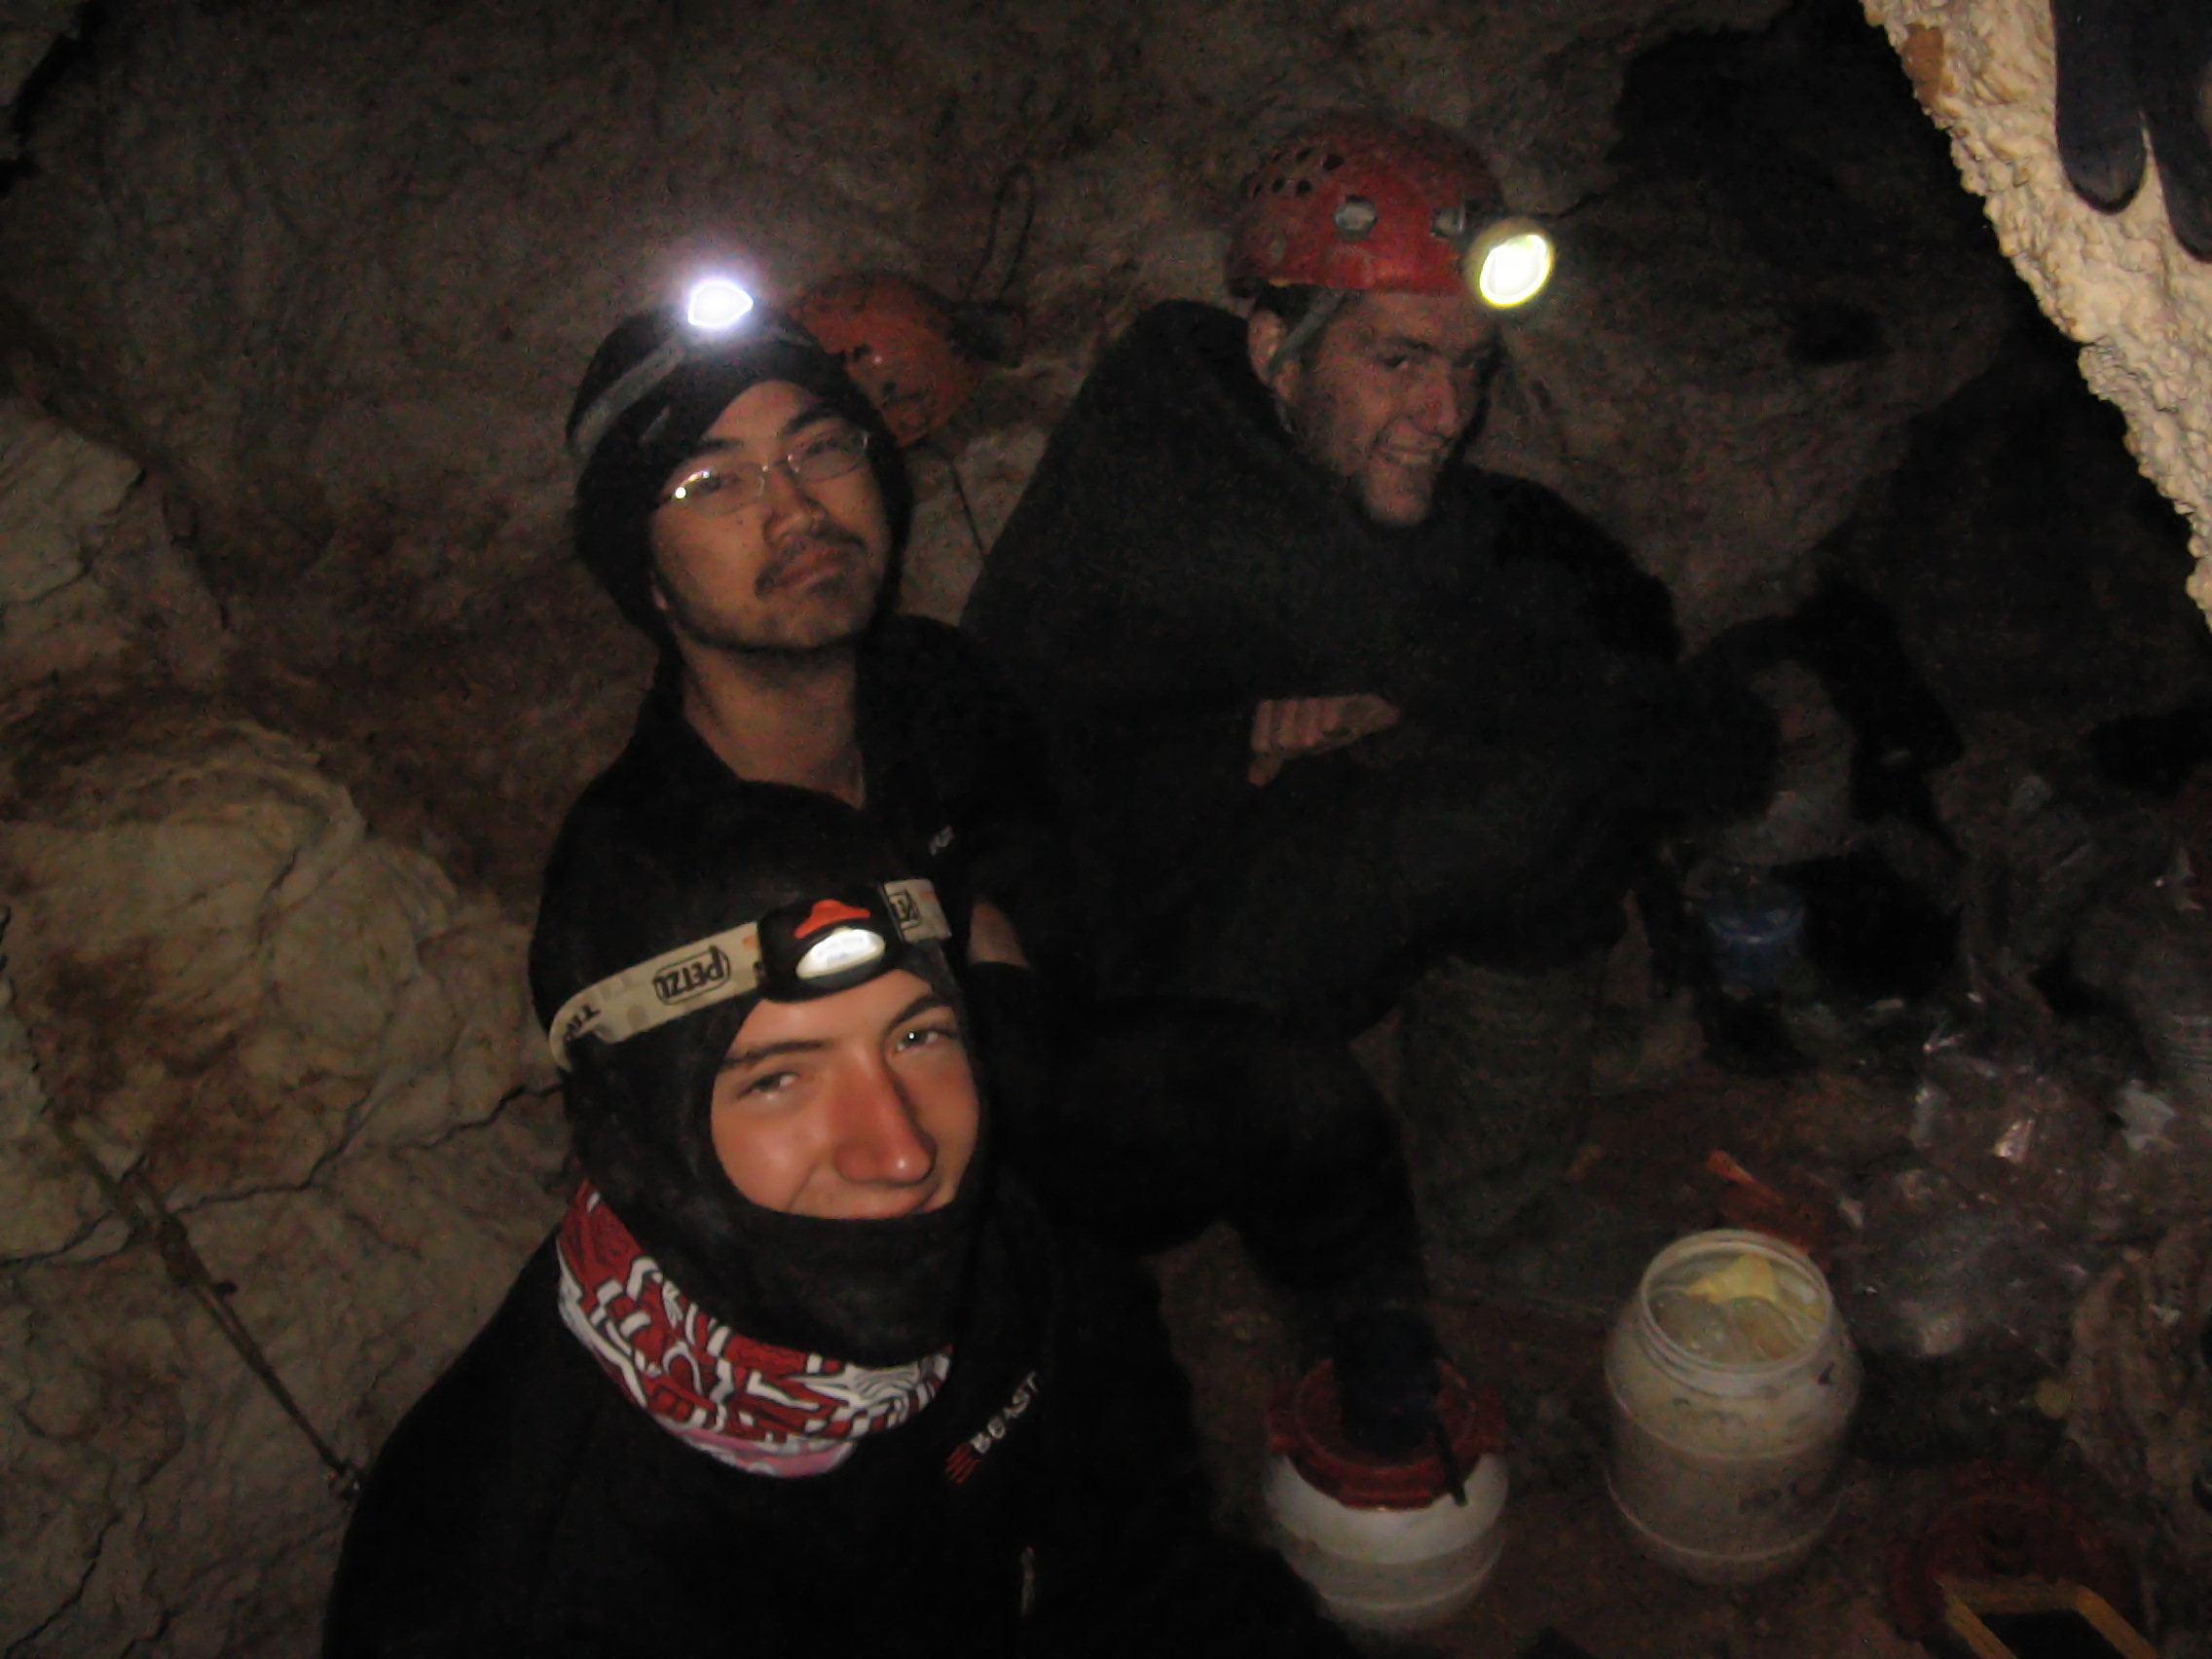
\includegraphics[width=\linewidth]{2009/63/2009-08-08-10.39.16 - Jana Carga - Canon Powershot A520 - Team Beast at Camp-GREYCstoration--orig.jpg}} 
 \caption{Tim, Thara and Dan at camp. \pic{Jana \v{C}arga}}
 \label{Thara Tim Dan Metal}
\end{marginfigure}

\margininbox{I Walk the Line}{
     \begin{itemize}
    \item Tim Osborne
    \item Tharatorn Supasiti
    \end{itemize}}{\explo}

We were supposed to be on a night train team following Tim and Thara. But
after spending a day quite active (caving and a carry) we decided to go
down in an early morning. Set an alarm for 5 am and start caving at 6.30
am. Down in the camp we woke the day team Tim and Thara. After breakfast
and a chat we swop the BEAST comf and go back to sleep. Thara and Tim
continue pushing the lead, which is still going. They come back at 10 am
and woke us up. Our first time sleeping in a camp was quite broken. For
the first 5-6 h we didn't really sleep. We also put extra extra comf in
our sleeping bags -- it was cold!

Tim and Thara pushed the cave for 2 pitches down: 10 m and 34 m.
Afterwards there is a climb up a boulder choke where they stopped. So we
went up, where on the other side was a pitch down. We spend two hours
rigging and gardening. Basically there are rocks and boulders all around
the pitch head. Going up and down was still dangerous -- stones
constantly falling down. Needed to be re-rigged. The way on then
continued up and into another smaller boulder choke. Under there was a
small pitch down. From there we first climb up the rock and end up above
big black hole. We throw a stone down and we can hear that there was a
long way down -- 4 seconds! Fucking hell -- that is like 80 m pitch.
\bignote{Very excited we keep on throwing stones down}. The echo at the bottom was
amazing. We could also hear that there was a big slope at the bottom.
From here the rigging down was not really good. So we looked for a
alternative way into a pitch. Further down there is a rift, which you
climb into it and it takes you straight to the pitch -- beautiful place
to bolt. Here we decided to survey from here back to the passage \passage{Walk the Line}.


\begin{figure}
\checkoddpage \ifoddpage \forcerectofloat \else \forceversofloat \fi
\frame{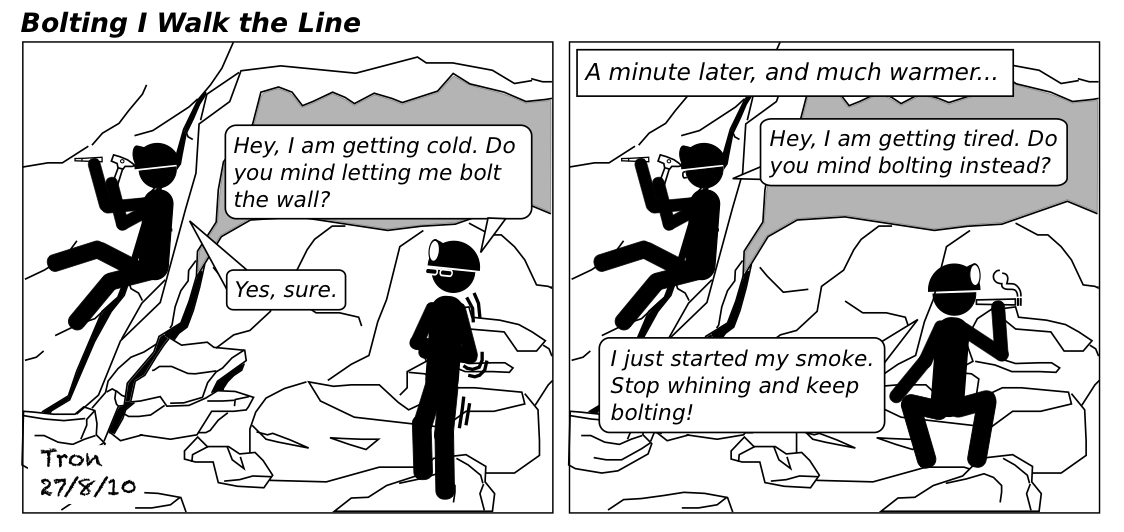
\includegraphics[width=\linewidth]{2009/63/Tharatorn Supasiti - March 2012 - walk-the-line--orig.jpg}}
\caption{The bolting of \passage{I Walk the Line}. \pen{Tharatorn Supasiti}}
\label{walk the line cartoon}
\end{figure}

\margininbox{For Evans' Sake, 2010}{
     "Jana Čarga for her 'goldfish from the fayre' production at underground camp, Slovenia, when using the composting toilet bags."}{\award}

Back in the camp after around 12h of caving.

Tim and Thara finish their caving in \passage{Gardeners' World} and went
back out. Alone in the cave we had to set up an alarm. We were woken up
by Tjaša, Izi and Erik, who were on a day trip to do some climbing in
\passage{Primula}. We re-start the alarm like 3 times and in the end end up
15h in bed! We finally got up at 5 am and start caving at 7.30 am. We
were excited, finally going down the big pitch and to see how big it
really is. We took two bolting kits to speed up. I spend time re-rigging,
bolting and more gardening below \passage{Walk the Line} and Dan went down to
start bolting the big pitch. After 3 hours we were ready to descend. Dan
offered me to go down first. I was ready to go and looking down was just
a bit scary, plus not having practice in dealing with enormous pitches I
thought would be better if Dan goes down first. He made another bolt
approx half way down on a tiny ledge. When he come down he shouted -- \bignote{O,
my god, it is really big!} Quickly followed down, looking around on the
way - Amazing!

\begin{figure*}[t!]
\checkoddpage \ifoddpage \forcerectofloat \else \forceversofloat \fi
\frame{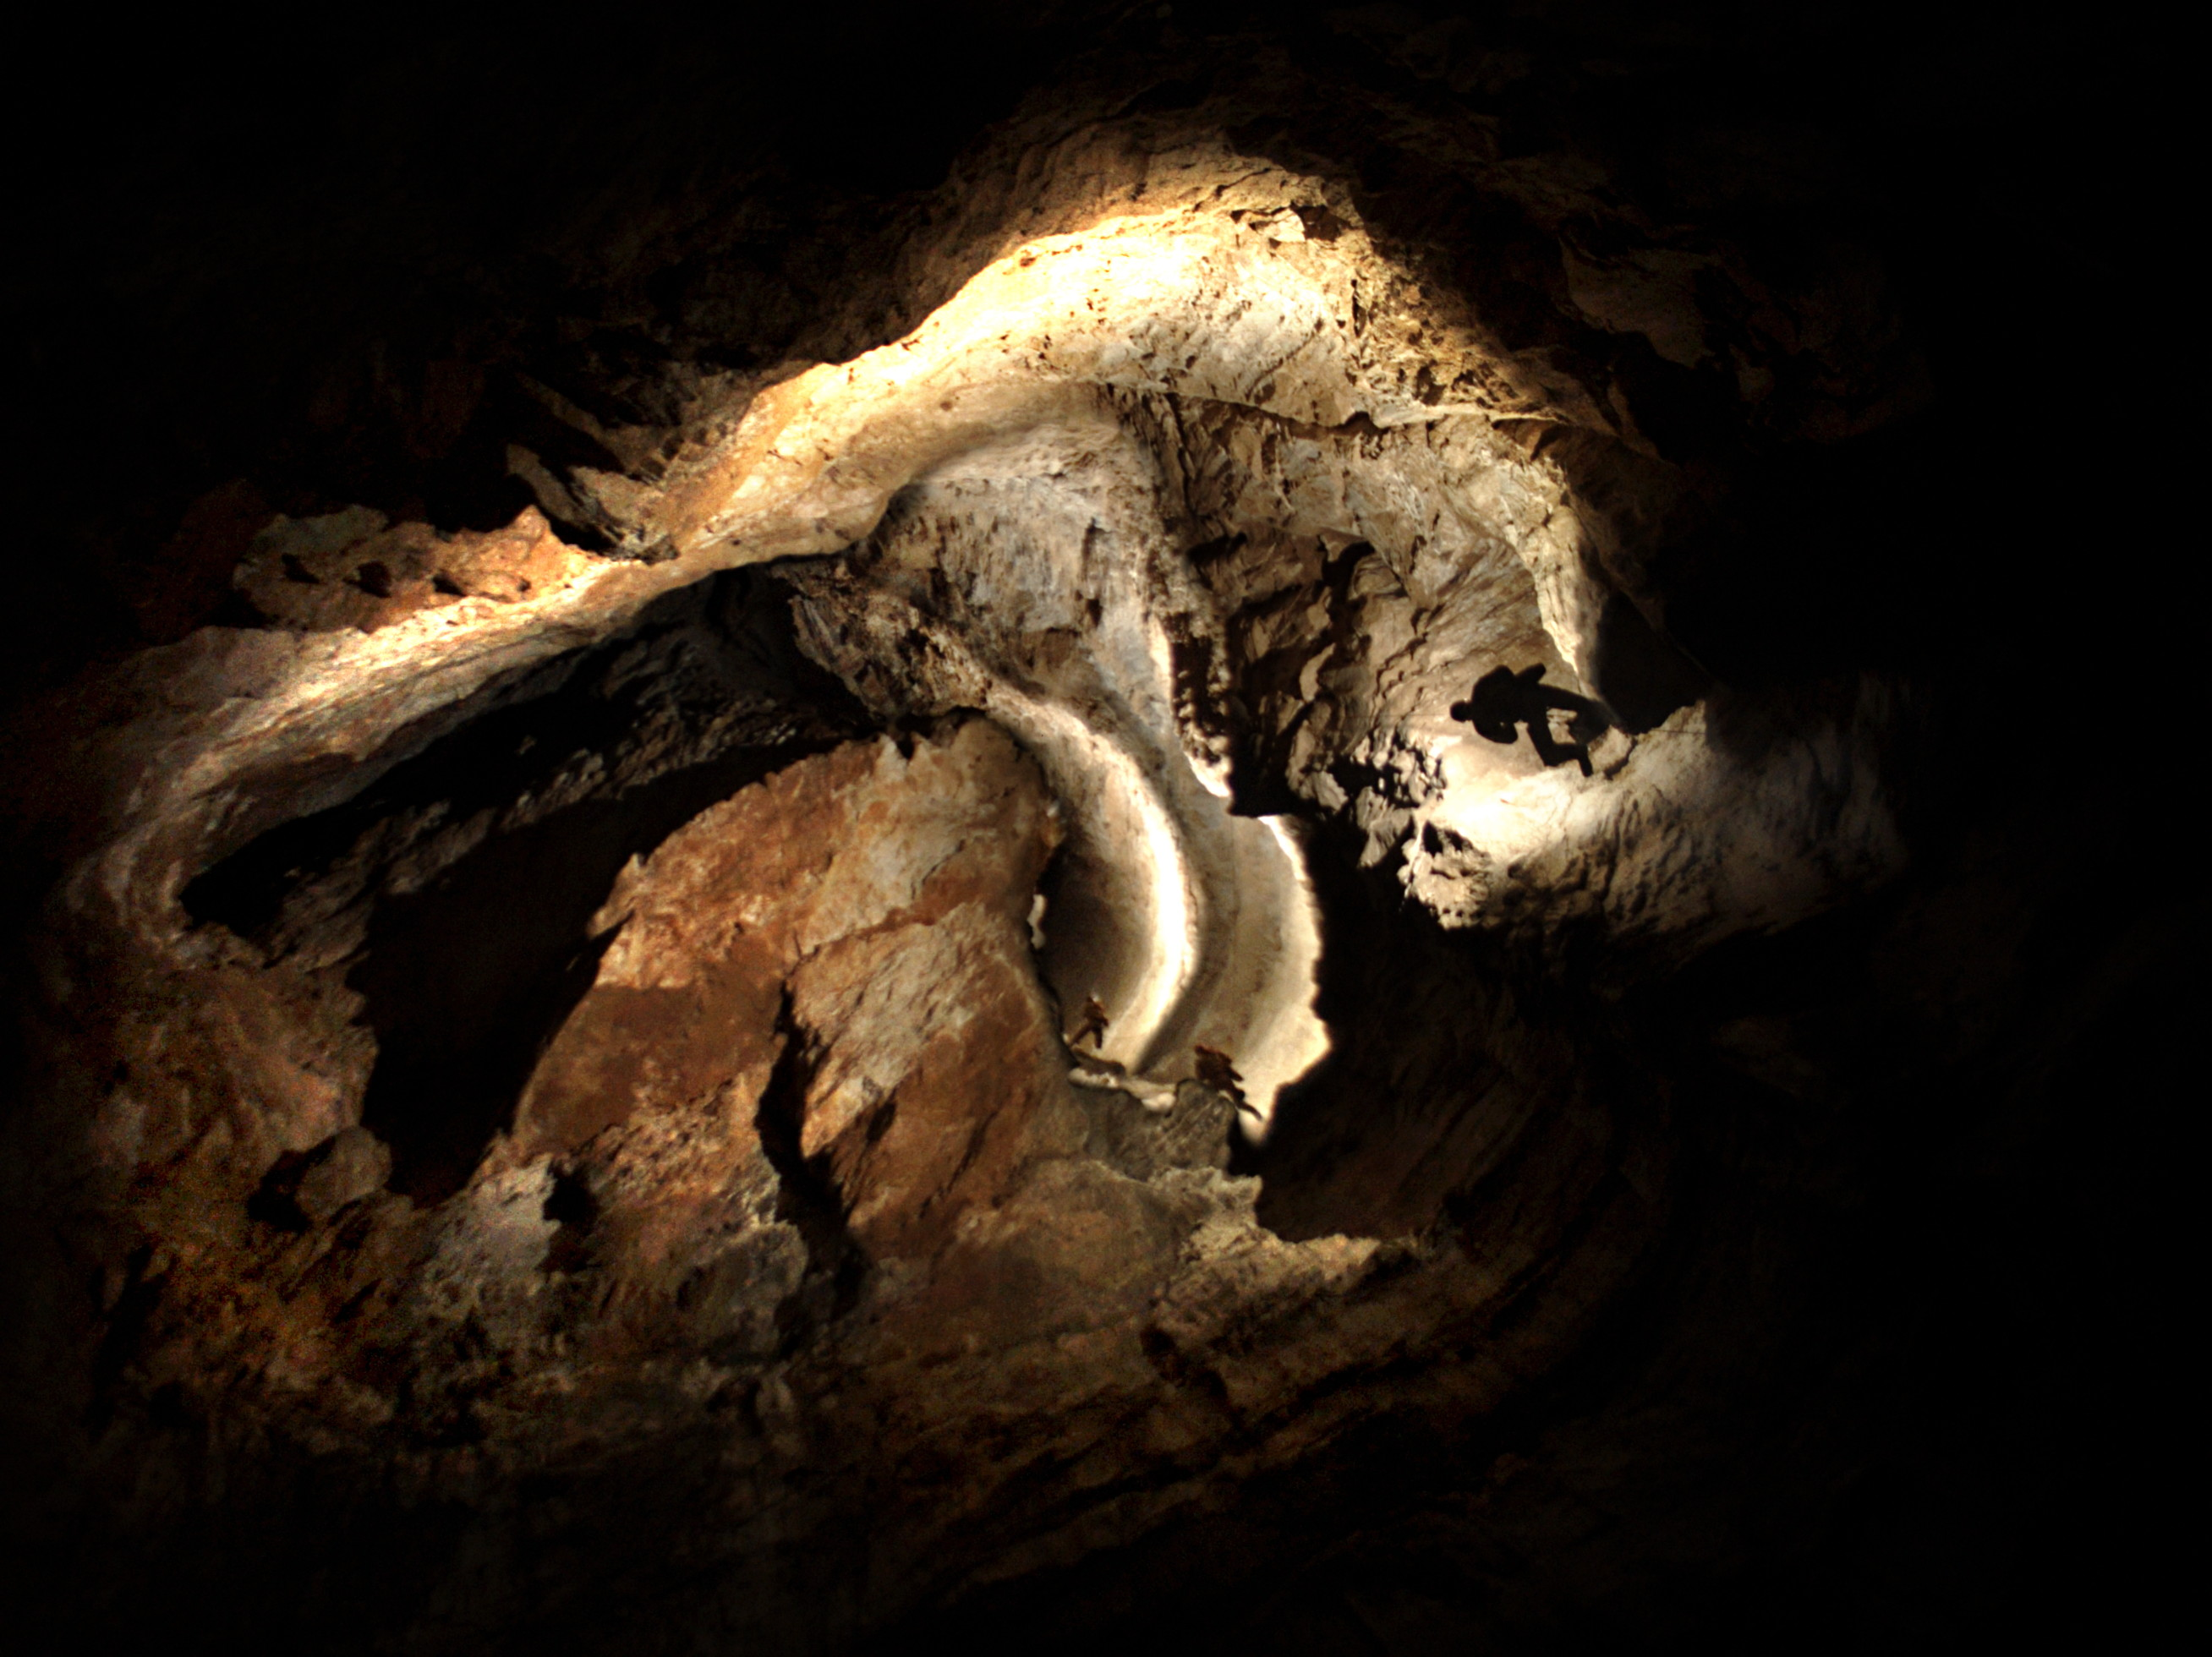
\includegraphics[width=\linewidth]{2009/63/2009-08-16-17.36.18 - Jarvist Frost - Canon Powershot G5 - happy monday pitch montage--orig.jpg}}
\caption{A composite photograph of Dan Greenwald ascending \protect\passage{Happy Monday}. \pic{Jarvist Frost}}
\label{happy monday pitch}
\end{figure*}


\begin{figure*}[t!]
\checkoddpage \ifoddpage \forcerectofloat \else \forceversofloat \fi
\centering
    \begin{subfigure}[t]{0.393\textwidth}
        \centering
        \frame{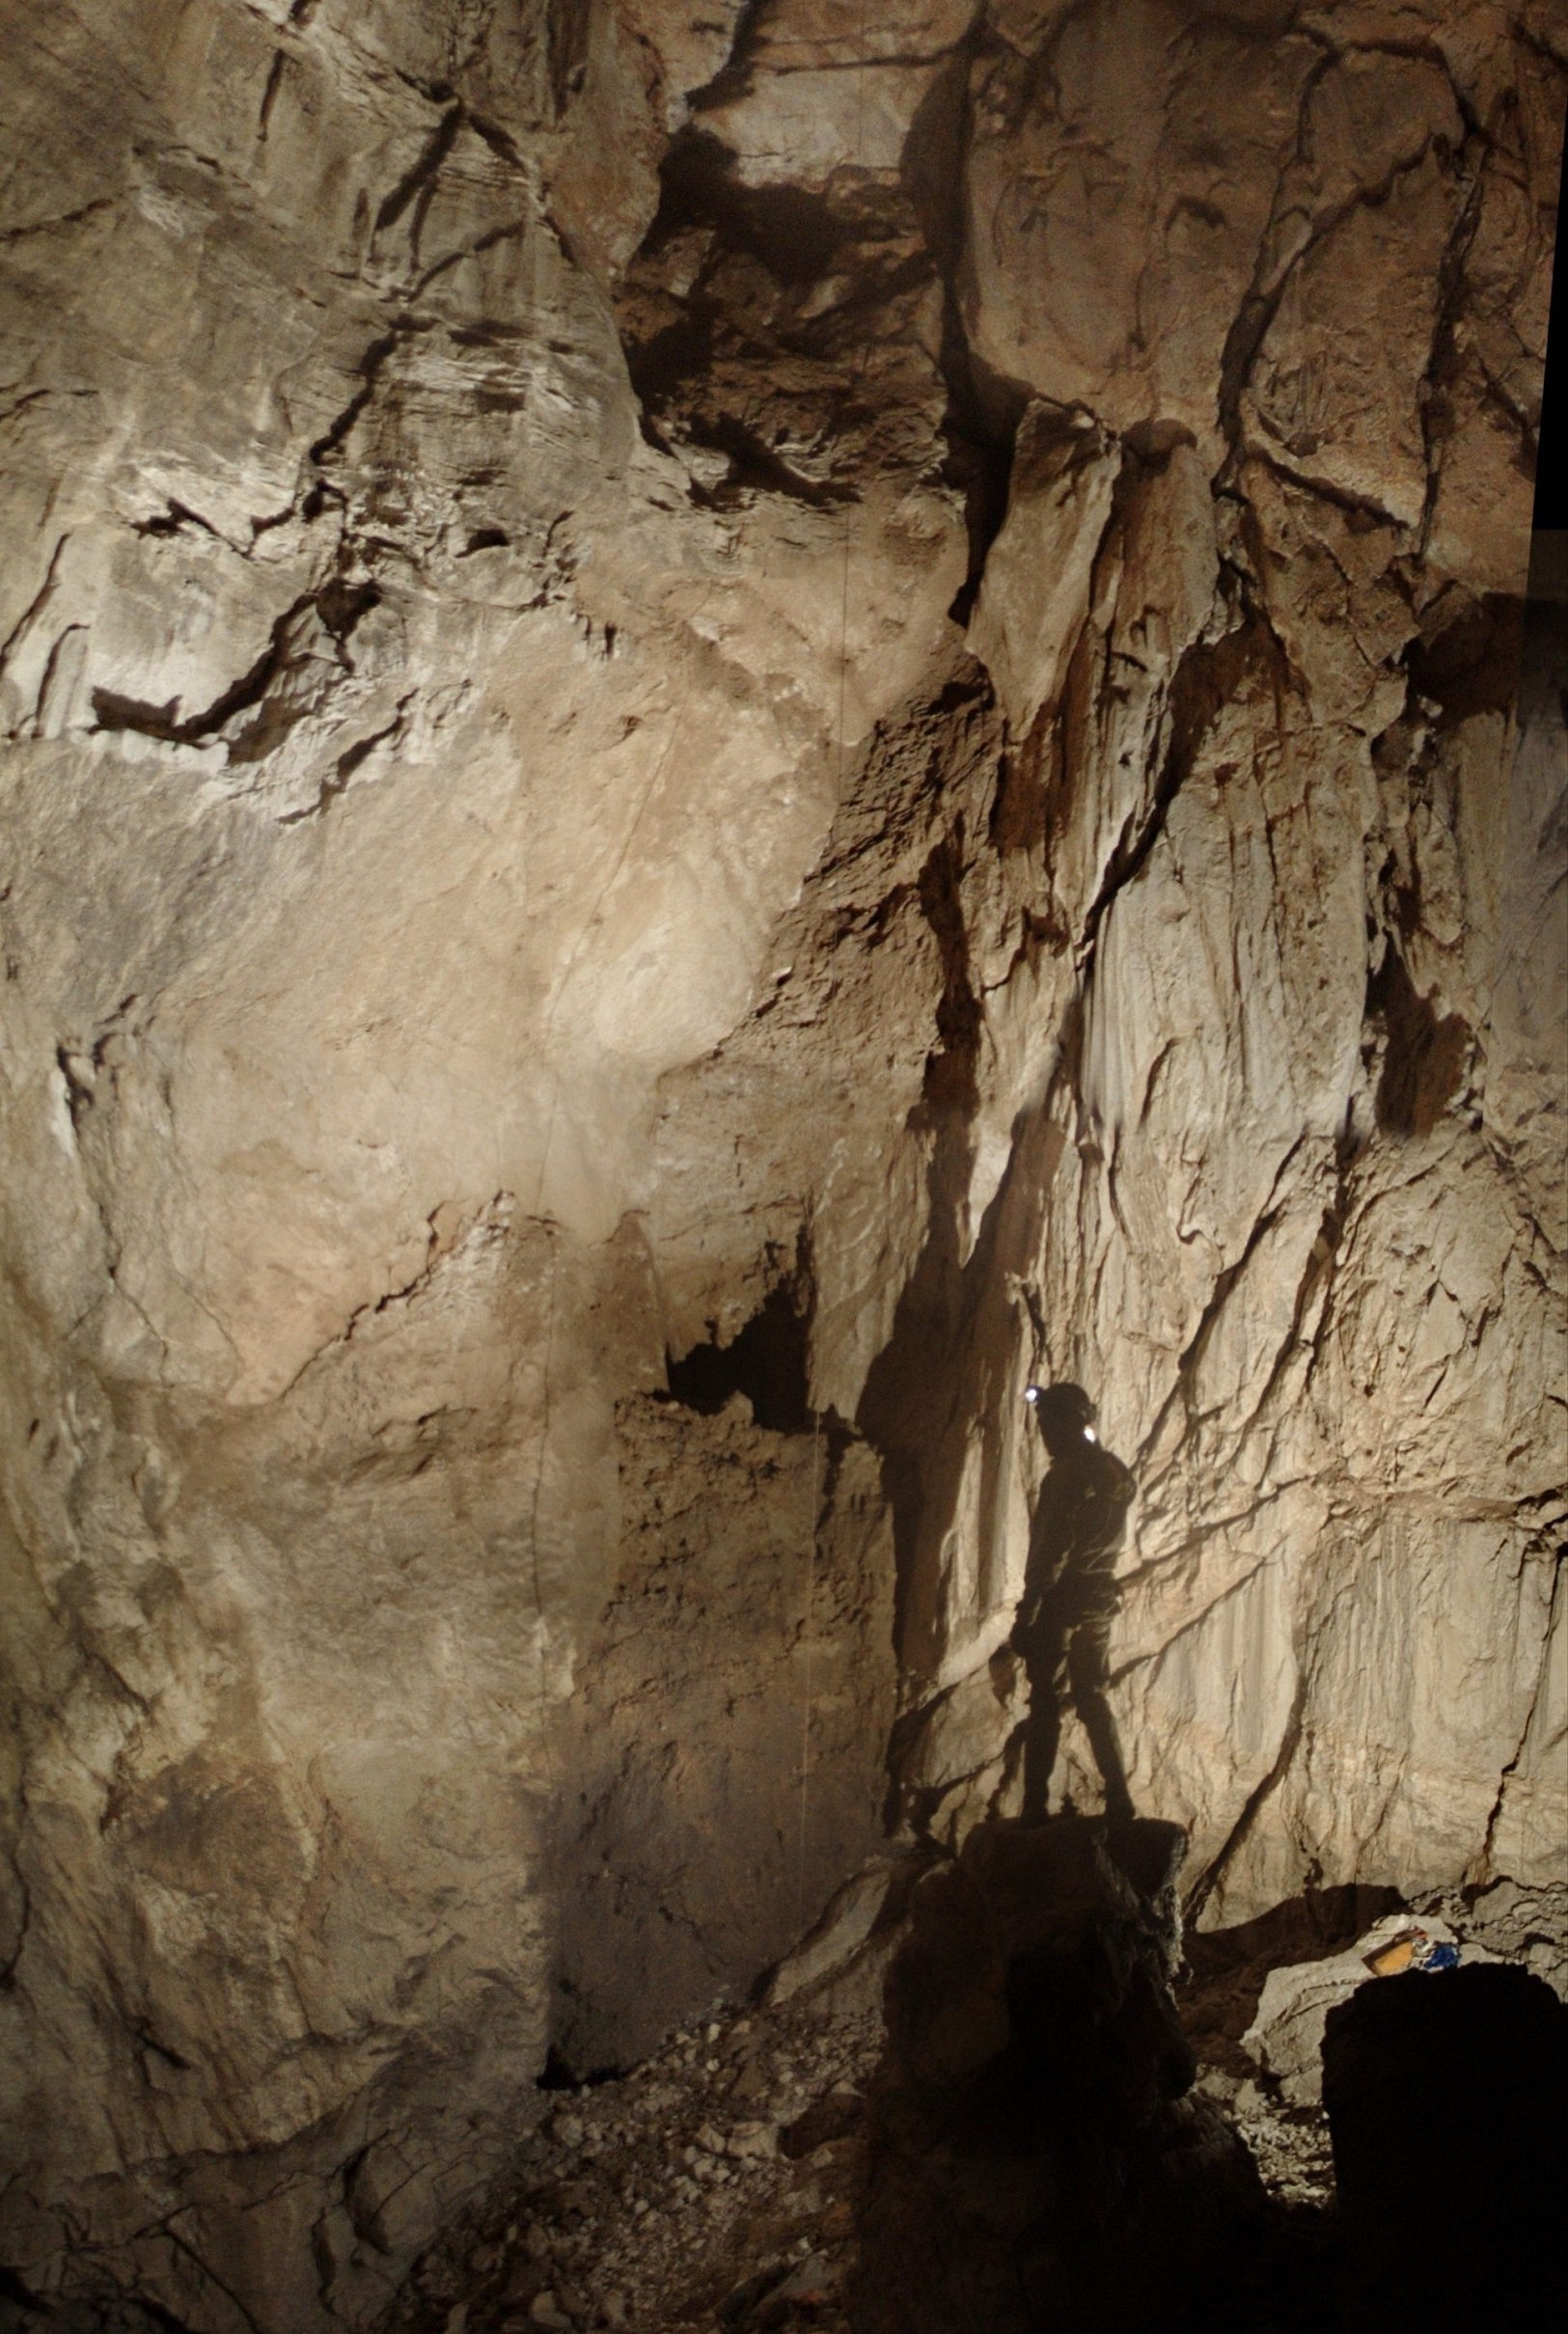
\includegraphics[width=\linewidth]{2009/63/happy monday base jarvist.jpg}} 
        \caption{} \label{happy monday base}
    \end{subfigure}
        \hfill
\begin{subfigure}[t]{0.59\textwidth}
\centering
\frame{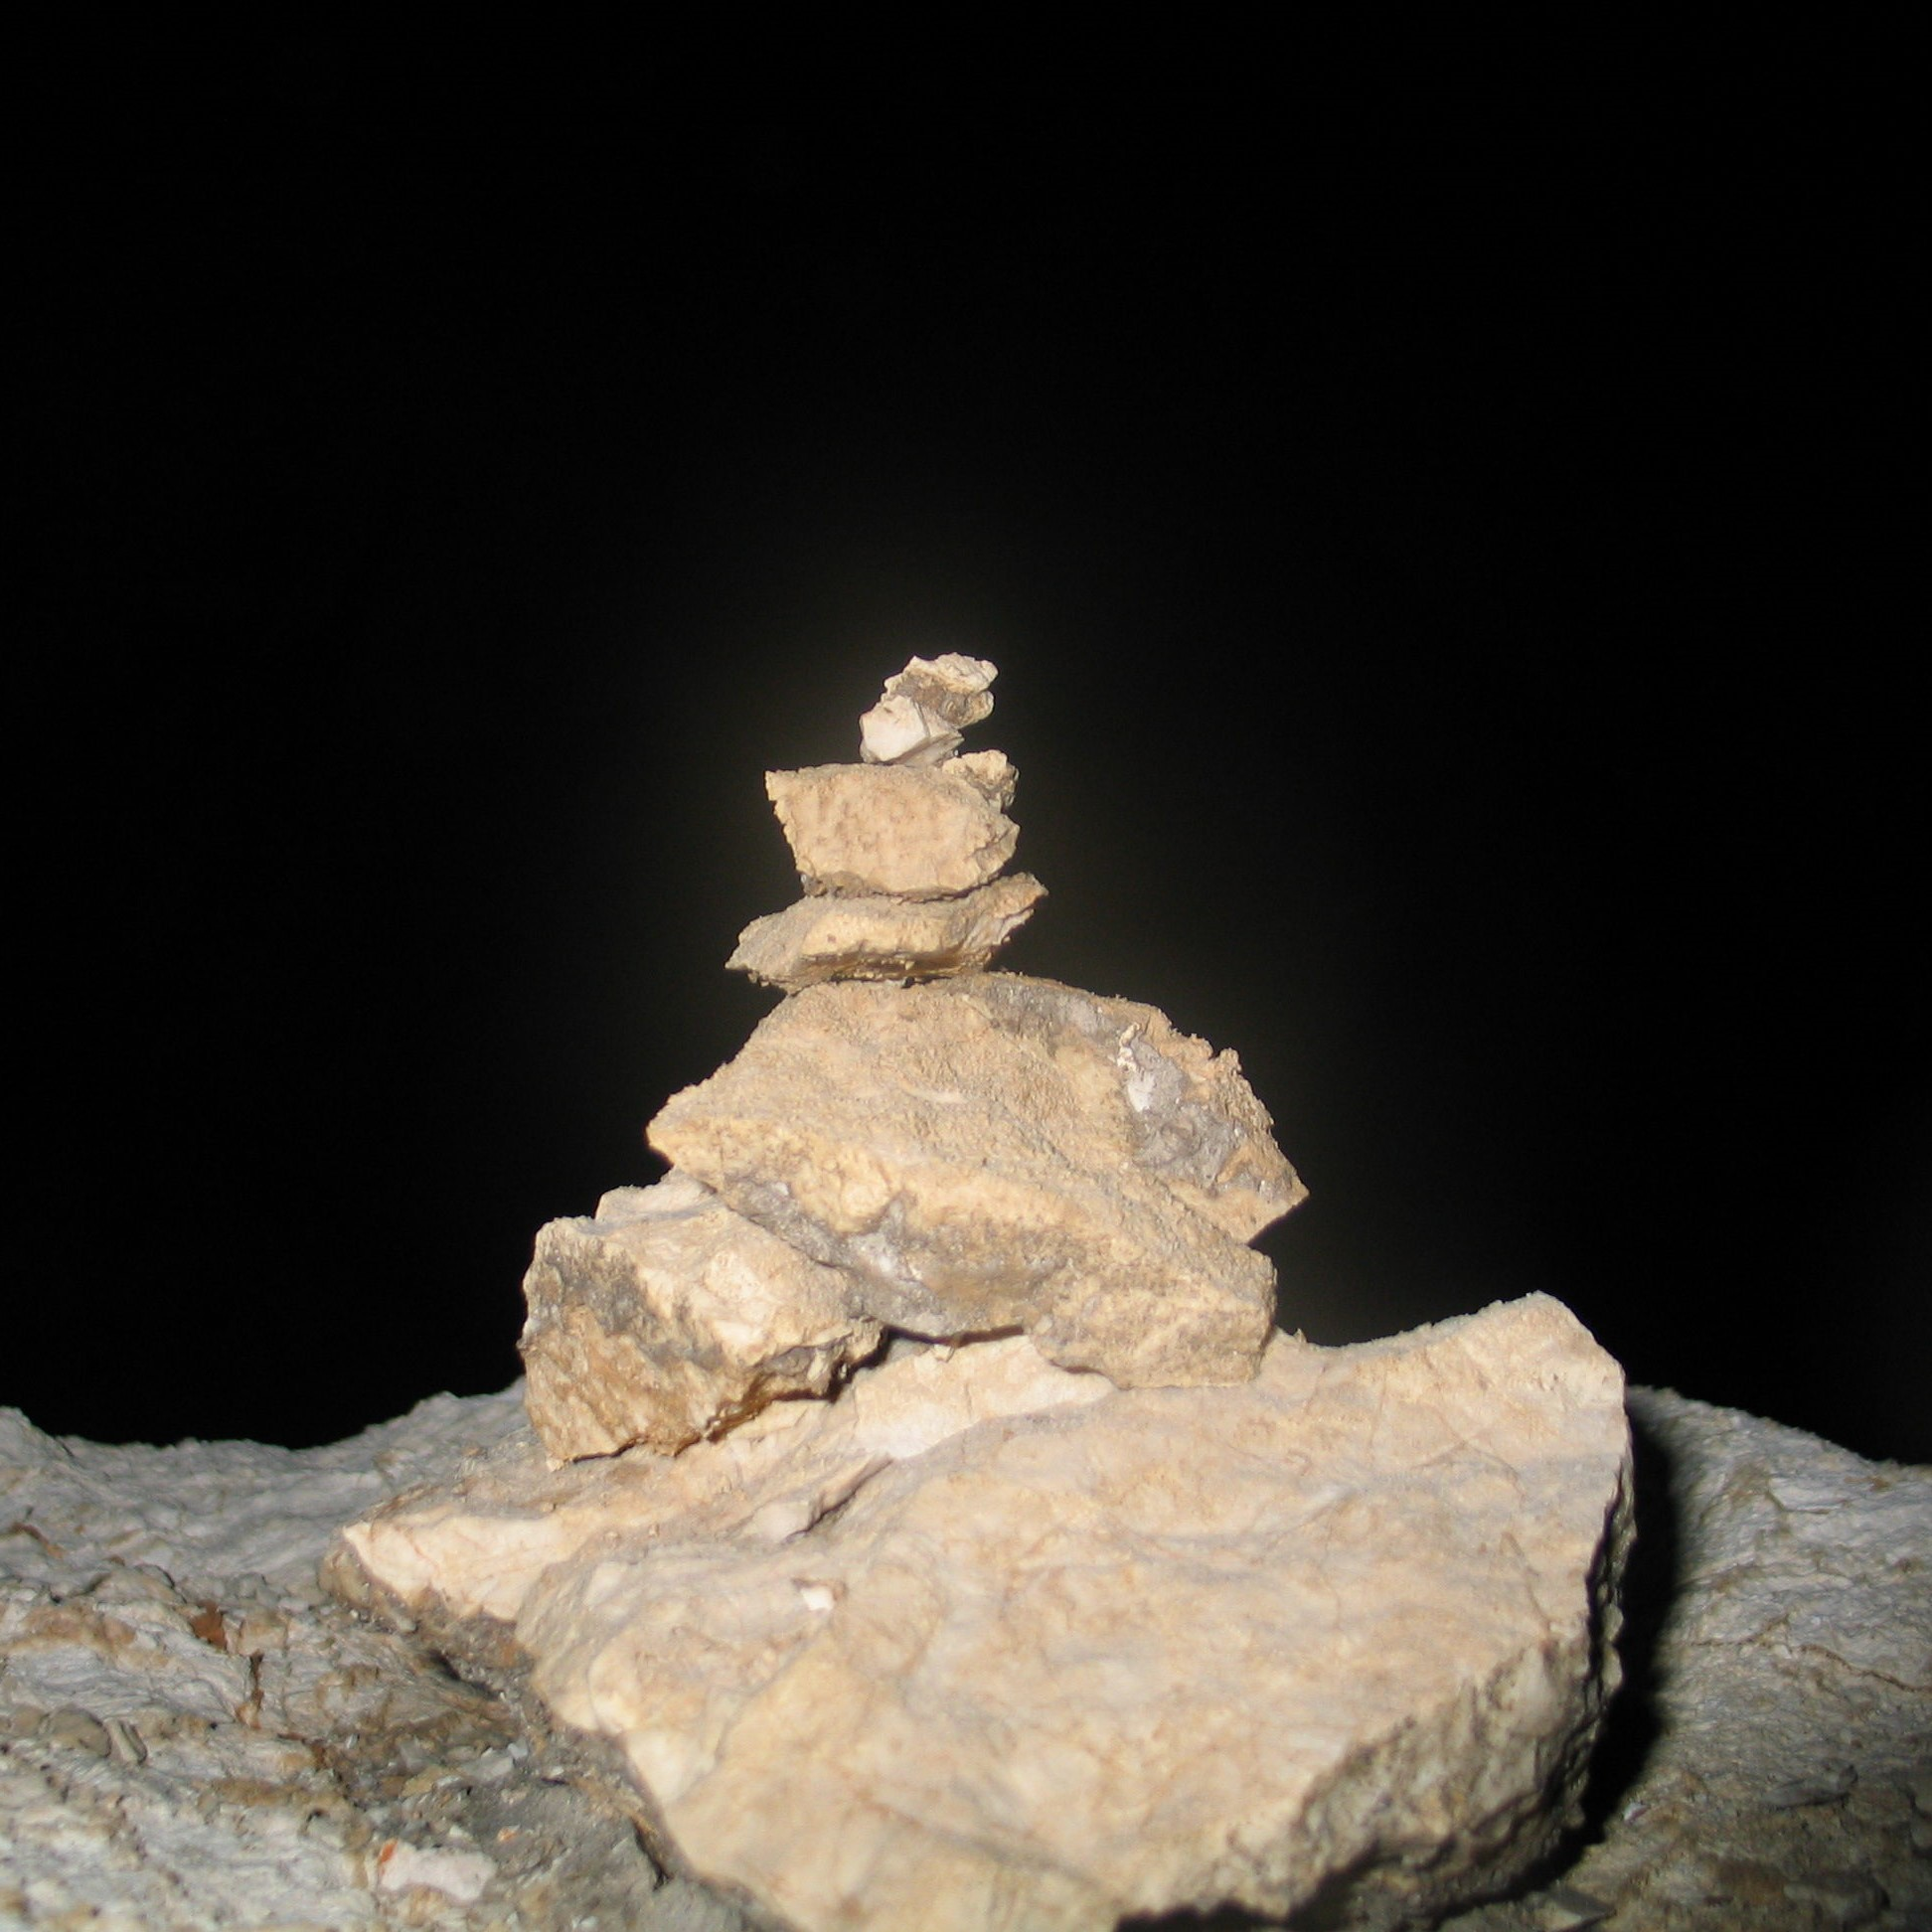
\includegraphics[width=\linewidth]{2009/63/2009-08-16-17.15.42 - Jarvist Frost - Canon Powershot G5 - Happy Monday - PSS Zero on standing stone--orig.jpg}}
 \caption{}\label{happy monday pss}
\end{subfigure}
    \vspace{0cm}
    \begin{subfigure}[t]{\textwidth}
    \centering
        \frame{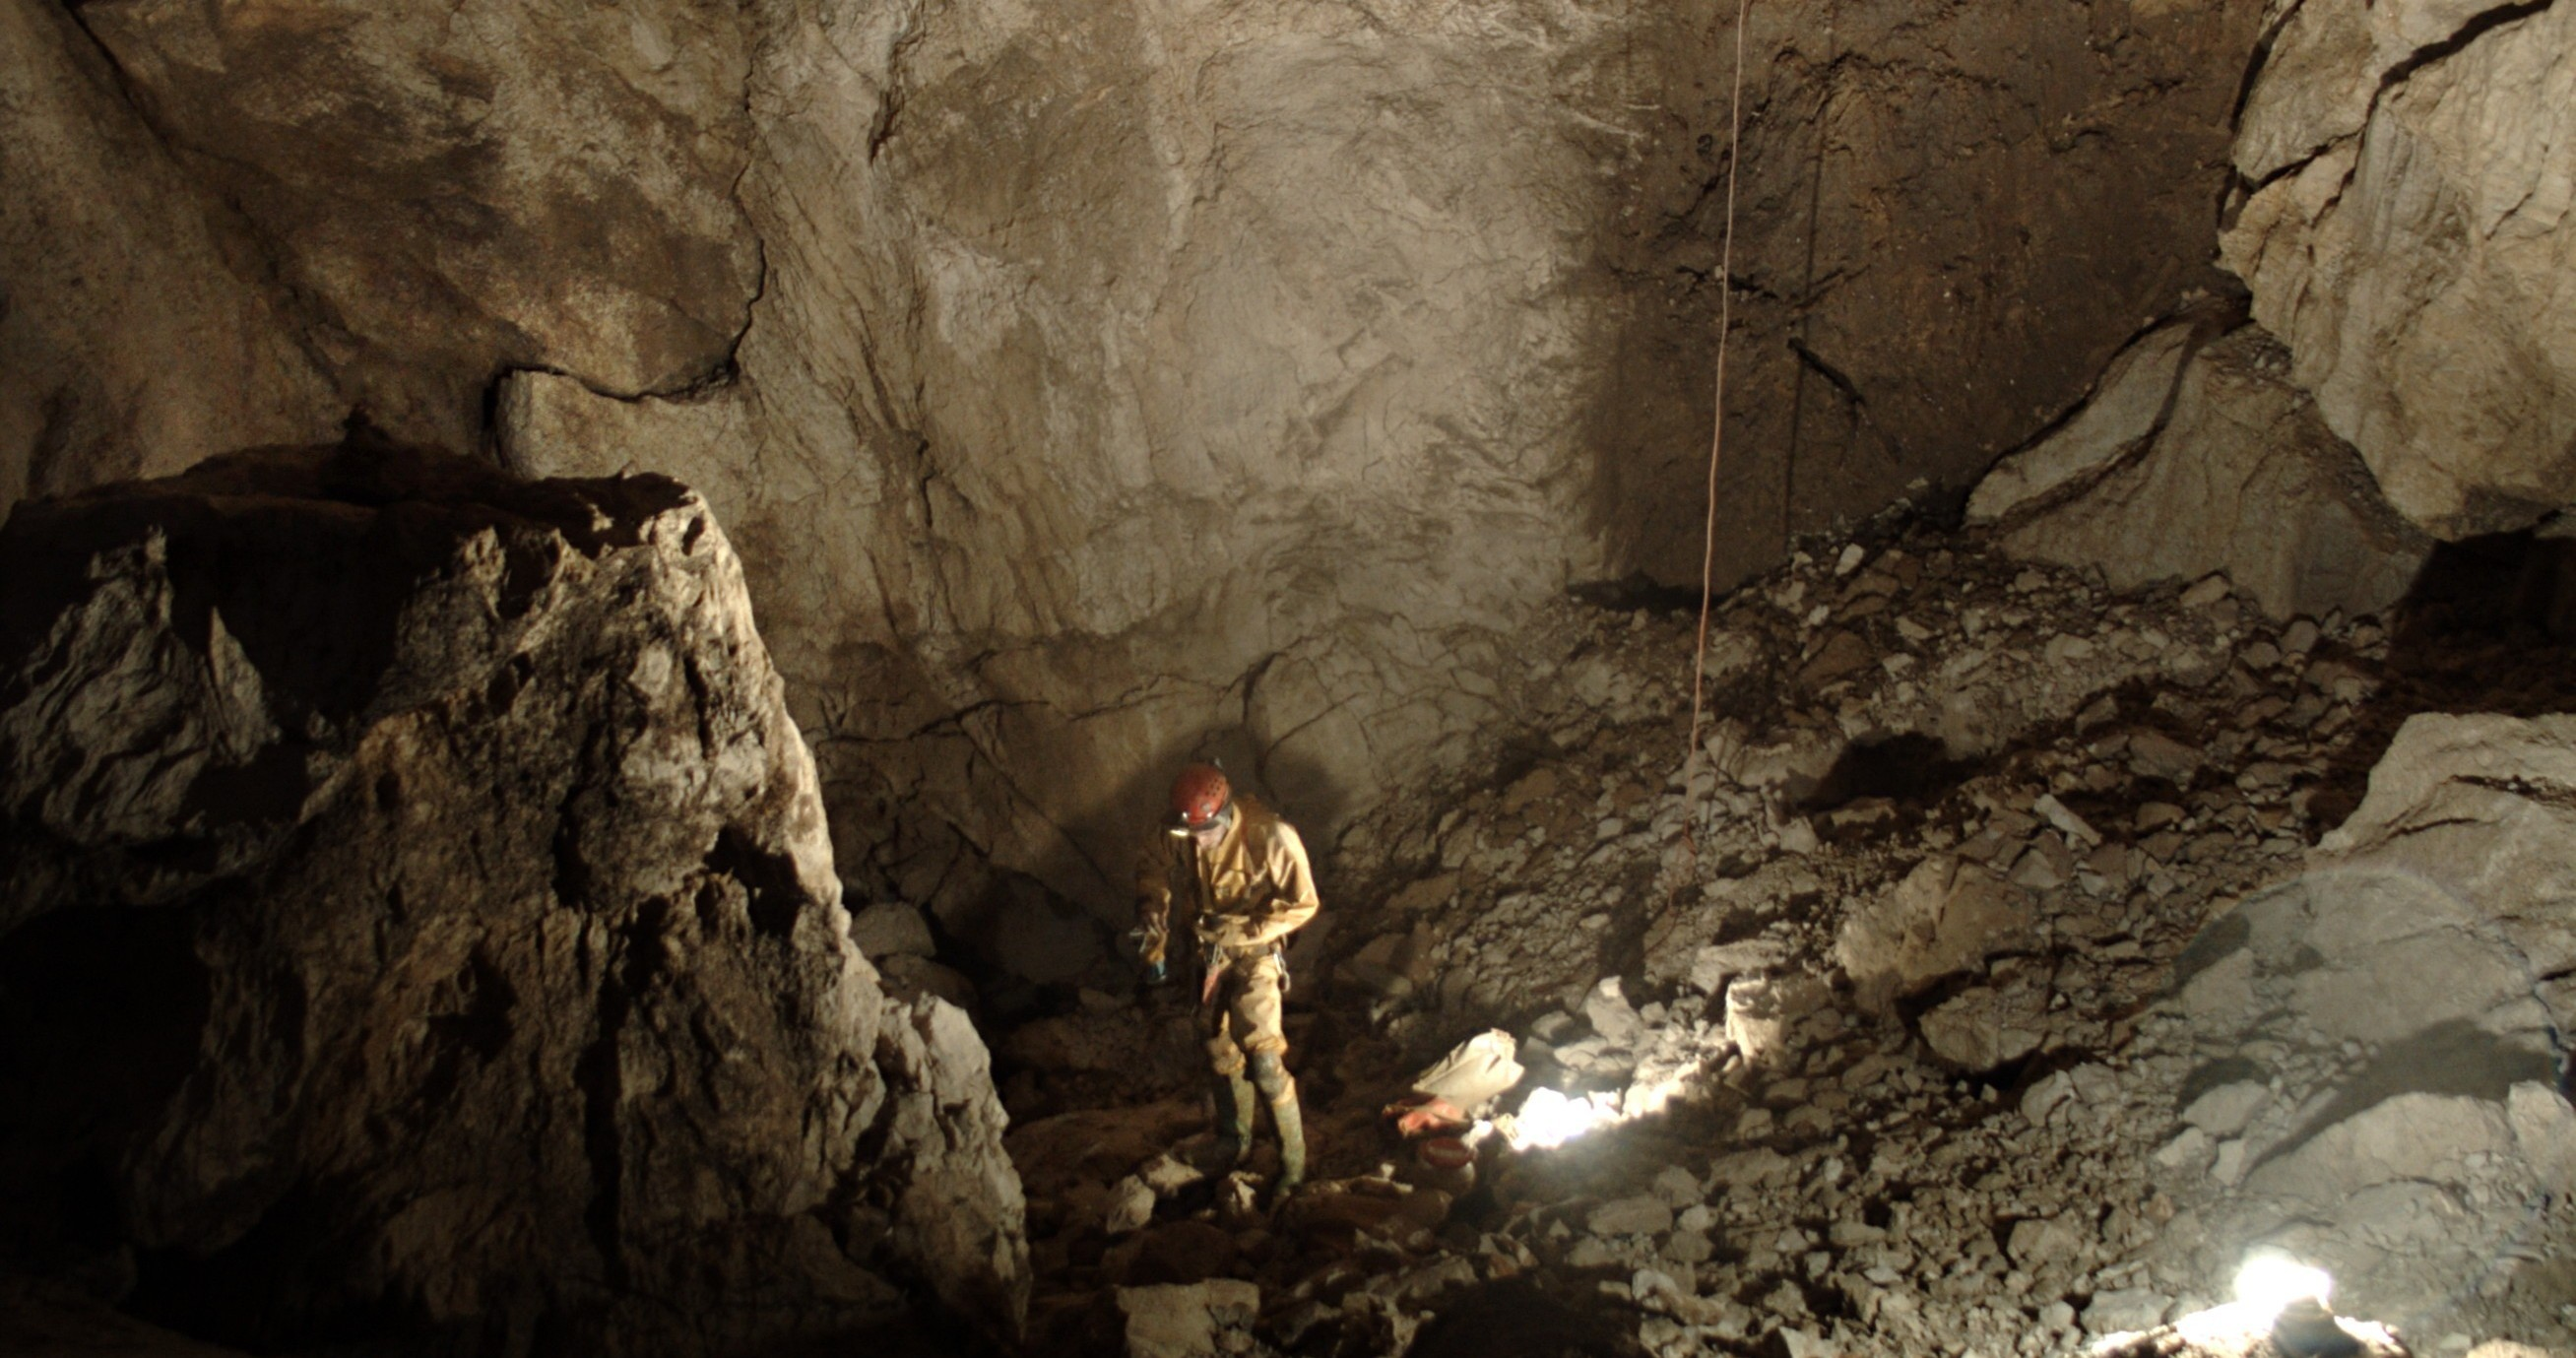
\includegraphics[width=\linewidth]{2009/63/2009-08-16-17.10.14 - Jarvist Frost - Canon Powershot G5 - happy monday - fettling at bottom2--orig.jpg}} 
        \caption{} \label{happy monday fettle}
    \end{subfigure}
    \caption{
    \textit{(a)} Dan on the standing stone below \protect\passage{Happy Monday} pitch.  
     \textit{(b)} Permanent Survey Station Zero.
     \textit{}{(c)} The base of \protect\passage{Happy Monday}. \pic{Jarvist Frost}}     \label{happy monday}
\end{figure*}

At the bottom we explored around and found the way on
under the boulder choke. There is another approx 10 m pitch on. We had
some lunch and then was time to survey it. The bottom was impressive:
\(20\times20\) m. Cuz the tape was not long enough we had to mark the
rope, using a zinc-oxide tape twice on a way up. The length to the
rigging spot was 75+15 m to the top. And there it was - a 90 m pitch.

Pleased with our mission we had to speed up to get out on time. Our call
out was 10 pm. We stopped in \passage{Metal camp} for hot chok and to
pack the stuff to be taken out. We were out from the bottom in 6h. Back
in the bivy at 9.45 pm.

We had a great trip and it was first time for both of us to be
underground for so long and to discover such a big pitch -- which still
does not have a name.

The next day, during the breakfast time we decided to name it:
\passage{Happy Monday}. \name{Jana \v{C}arga}
